\documentclass{letter}
\usepackage[margin=0.75in]{geometry}
\usepackage{amsmath}
\usepackage{amssymb}
\usepackage{enumerate}
\usepackage{changepage}
\usepackage{tikz}
\usepackage{pgfplots}
\pgfplotsset{compat=1.8}

\pgfplotsset{vasymptote/.style={
		before end axis/.append code={
			\draw[densely dashed] ({rel axis cs:0,0} -| {axis cs:#1,0})
			-- ({rel axis cs:0,1} -| {axis cs:#1,0});
		}
	}}

\begin{document}
	\begin{center}
		\LARGE Math137 - December 02, 2015\\
		\large Areas Between Curves
	\end{center}
	\vspace{0.25 in}
	
	\begin{itemize}
		\item[\textbf{Ex. }] Find the area $A$, enclosed by the parabola $y = 2 - x^2$ and the line $y = -x$.\\\\
		To set up a definite integral between to curves, we need to know two things:
		\begin{itemize}
			\item The bounds of integration (Intersection points)
			\item We must know which function is on top.
		\end{itemize}
		
		First, lets find our intercepts so we can find what area is enclosed.
		\begin{flalign*}
			2-x^2 &= -x&\\\
			0 &= x^2 - x - 3\\
			&= (x-2)(x+1) 
		\end{flalign*}
		
		$\therefore$ our bounds are -1 $\to$ 2, $a= -1, b = 2$.\\\\
		To find which function is on top, we should do a sketch since these are easy polynomials. Notice below, for the enclosed area, the parabola is on top. We could also have tried a test value in the interval to see which produces a higher $y$ value.\\\\
		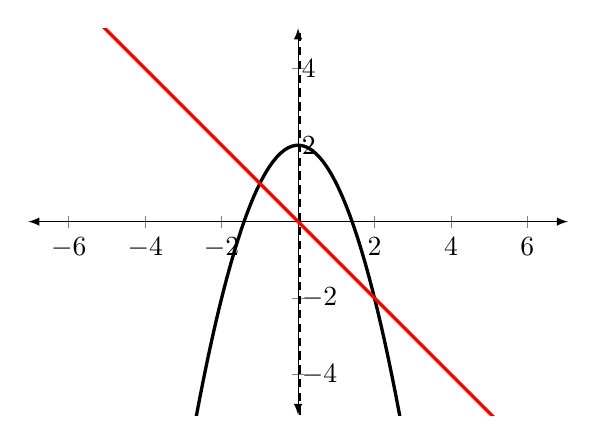
\begin{tikzpicture}
		\begin{axis}[
		axis equal image,
		axis lines=middle,
		xmin=-5,xmax=5,
		ymin=-3,ymax=3,
		enlargelimits={abs=1cm},
		axis line style={latex-latex},
		yticklabel style={anchor=west},
		vasymptote=0.05,
		]
		% This doesn't clip to y=-10:10 nicely
		% because there are too few samples near the asymptote:
		\addplot[very thick, black, domain=-10:10,samples=200, restrict y to domain=-10:100]
		{2 - x^2};
		\addplot[very thick, red, domain=-10:10,samples=200, restrict y to domain=-10:100]
		{-x};
		\end{axis}
		\end{tikzpicture}
		\begin{flalign*}
			A &= \int_{-1}^{2} \left[ (2-x^2) - (-x) \right] dx&\\
			&= \int_{-1}^{2} \left[ -x^2 + x + 2\right]\\
			&= \left[ \frac{-1}{3}x^3 + \frac12 x^2 + 2x \right]_{-1}^2\\
			&= (4-\frac83 + 2) - (2 + \frac13 + \frac12)\\
			&= \frac92
		\end{flalign*}
		\clearpage
		\item[\textbf{Ex. }] Find the area $A$ bounded by the curve $y = x^3 + x^2$ and the line $y = 2x$.\\\\
		The cubic graph isn't super straight forward, so lets figure out our bounds first and see if we can make some assumptions by that.
		\begin{flalign*}
			x^3 + x^2 &= 2x&\\
			x^3 + x^2 - 2x &= 0\\
			x(x+2)(x-1) &= 0
		\end{flalign*}
		So we have roots at -2, 0 and 1. We also know the cubic is positive, so we can probably make a pretty good estimate of the graph of this function.\\\\
		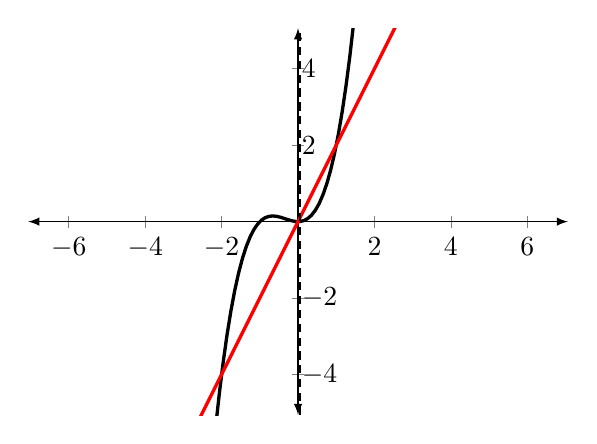
\begin{tikzpicture}
		\begin{axis}[
		axis equal image,
		axis lines=middle,
		xmin=-5,xmax=5,
		ymin=-3,ymax=3,
		enlargelimits={abs=1cm},
		axis line style={latex-latex},
		yticklabel style={anchor=west},
		vasymptote=0.05,
		]
		% This doesn't clip to y=-10:10 nicely
		% because there are too few samples near the asymptote:
		\addplot[very thick, black, domain=-10:10,samples=200, restrict y to domain=-10:100]
		{x^3 + x^2};
		\addplot[very thick, red, domain=-10:10,samples=200, restrict y to domain=-10:100]
		{2*x};
		\end{axis}
		\end{tikzpicture}\\\\
		Uh oh, two separate areas. This means we need to use two integrals to calculate the area, and them sum them. We need to use to two different integrals because which polynomial is on top changes at the point (0, 0), and the order of subtraction matters.\\
		Let the lower area be equal to $A_1$. Let the upper area be equal to $A_2$. $A = A_1 + A_2$\\\\
		\begin{minipage}[t]{0.5\textwidth}
			\underline{$A_1$}
			\begin{flalign*}
				&\int_{-2}^{0} \left[(x^3 + x^2) - (2x)\right] dx&\\
				&= \int_{-2}^{0} \left[ x^3 + x^2 - 2x\right] dx\\
				&= \left[ \frac{x^4}{4} + \frac{x^3}{3} - x^2\right]_{-2}^0\\
				&= 0 - (4 - \frac83 - 4)\\
				&= \frac83
			\end{flalign*}
		\end{minipage}
		\begin{minipage}[t]{0.5\textwidth}
			\underline{$A_2$}
			\begin{flalign*}
				&\int_0^1\left[(2x) - (x^3 + x^2)\right] dx\\
				&= \int_0^1 \left[ -x^3 -x^2 + 2x\right] dx\\
				&= \left[ -\frac{x^4}{4} - \frac{x^3}{3} + x^2\right]_0^1\\
				&= -\frac14 -\frac13 + 1 - 0\\
				&= \frac{5}{12}\\
			\end{flalign*}
		\end{minipage}\\
		
		$A = A_1 + A_2$\\
		$A = \dfrac83 + \dfrac{5}{12}$\\
		$A = \dfrac{37}{12}$\\
		\clearpage
		\item[\textbf{Ex. }] Find the area $A$ of the region bounded by the curves $y = 2 \cos x + 1$ and $y = 1 - 2\sin x$ from $x= 0$ to $x = \frac{3\pi}{4}$\\\\
		We'll start by finding the intersection.
		\begin{flalign*}
			2 \cos x + 1 &= 1 - 2 \sin x&\\
			\cos x &= - \sin x\\
			1 &= -\tan x \;\;\;\; (x \neq \frac{\pi}{2} + 2k\pi,\; k \in \mathbb{Z})\\
			\tan x &= 1\\
			x &= \frac{3 \pi}{4}
		\end{flalign*}\\
		
		By the graph below, we see $2\cos x + 1$ is above the other function.\\
		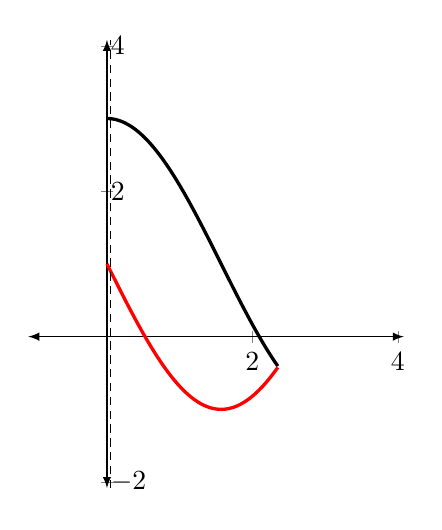
\begin{tikzpicture}
		\begin{axis}[
		axis equal image,
		axis lines=middle,
		xmin=0,xmax=3,
		ymin=-1,ymax=3,
		enlargelimits={abs=1cm},
		axis line style={latex-latex},
		yticklabel style={anchor=west},
		vasymptote=0.05,
		]
		% This doesn't clip to y=-10:10 nicely
		% because there are too few samples near the asymptote:
		\addplot[very thick, black, domain=0:2.35,samples=200, restrict y to domain=-10:100]
		{(2 * cos((x) r)) + 1};
		\addplot[very thick, red, domain=0:2.35,samples=200, restrict y to domain=-10:100]
		{1 - (2 * sin((x) r)))};
		\end{axis}
		\end{tikzpicture}\\
		\begin{flalign*}
			A &= \int_0^{3\pi / 4} \left[ (2 \cos x + 1) - (1 - 2 \sin x) \right] dx&\\
			&= \int_0^{3 \pi / 4} \left[2 \cos x + 2 \sin x \right] dx\\
			&= 2 \int_0^{3 \pi / 4}\left[ \cos x + \sin x \right] dx\\
			&=2 \left[\sin x - \cos x \right]_0^{3 \pi / 4}\\
			&= 2 \left[(\sin \frac{3 \pi}{4} - \cos \frac{3 \pi}{4}) - (\sin 0 - \cos 0)\right]\\
			&= 2(\frac{2}{\sqrt2} + 1)
		\end{flalign*}
	\end{itemize}
\end{document}